% -*- LaTeX -*-
% -*- coding: utf-8 -*-
%
% michael a.g. aïvázis
% california institute of technology
% (c) 1998-2012 all rights reserved
%

\lecture{Introduction to \pyre}{20120530}

% --------------------------------------
% the application harness
\begin{frame}[fragile]
%
  \frametitle{Creating an application}
%
  \python{firstnumber=10,linerange={10-35}}{listings/quad.py}
%
\end{frame}

% --------------------------------------
% the application harness
\begin{frame}[fragile]
%
  \frametitle{Auto-launching}
%
  instantiating and launching the application
%
  \python{firstnumber=55,linerange={55-60}}{listings/quad.py}
%
  a sample configuration file
%
  \cfg{firstnumber=8, linerange={8-20}}{listings/quad.cfg}
%
\end{frame}

% --------------------------------------
% the application component
\begin{frame}[fragile]
%
  \frametitle{The application component}
%
  quick introduction to pML 
%
  \begin{figure}
    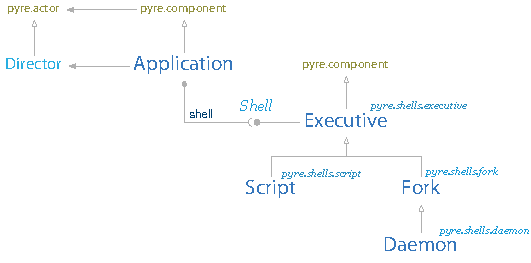
\includegraphics[scale=1.0]{figures/pyre-shells.pdf}
  \end{figure}
%
  our \identifier{Quad} derives from \identifier{Application}, so it has a \identifier{shell}
%
\end{frame}

% --------------------------------------
% the parallel version
\begin{frame}[fragile]
%
  \frametitle{Parallel integration}
%
  the \identifier{mpi} entry point
%
  \python{firstnumber=37,linerange={37-52}}{listings/quad.py}
%
  the \package{mpi} package is part of the pyre distribution
  \begin{itemize}
  \item handles initialization and finalization of \package{MPI}
  \item simplifies most of the ``overhead'' activities
  \item provides an OO veneer
  \end{itemize}
%
\end{frame}

% --------------------------------------
% running the mpi program
\begin{frame}[fragile]
%
  \frametitle{Running in parallel}
%
  minor modifications to the configuration file...
%
  \cfg{firstnumber=8, linerange={8-28}}{listings/quad.cfg}
%
\end{frame}

% end of file 
